%%%%%%%%%%%%%%%%%%%%%%%%%%%%%%%%%%%%%%%%%%%%%%%%%%%%%%%%%%%%%%%%
%%                                                            %%
%% aGreekPrimer, Italian translation 2016.12 - 2017           %%
%%                                                            %%
%% From:  Clarence W. Gleason, A Greek Primer                 %%
%%        (1903, New York, American Book Company)             %%
%%                                                            %%
%%        https://archive.org/details/greekprimer00glea       %%
%%                                                            %%
%% Translated by g.p.ciceri <gp.ciceri@gmail.com>             %%
%% ---------------------------------------------------------- %%
%% This translation is Licensed under                         %%
%% Creative Commons Attribution-ShareAlike 4.0 International  %%
%% https://creativecommons.org/licenses/by-sa/4.0/            %%
%%                                                            %%
%%%%%%%%%%%%%%%%%%%%%%%%%%%%%%%%%%%%%%%%%%%%%%%%%%%%%%%%%%%%%%%%

% ᾶῖῶῆῦ  
% ἀἰὐἐὀὠἠ 
% ὰὲὶὸὺὼὴ 
% ἁἱὑὁὡἡῥ
% άέίόύήώΆΉ
% ἂἒὒἲὂὢἢὒἚἊ
% ἃἳὓὃἣὣἓἋἛ
% ἄἔἴὄὔὤἤἌἬ
% ἅἕἵὅὕὥἥἍἭ
% ἆὦἶἦὖἯἏὯἇὧἷἧὗἯἏὯ 

% ᾳῃῳ
% ᾱῑῡ
% ᾀᾐᾠ
% ᾰῐῠ
% ᾂᾒᾢ
% ϊ ϋ
% ᾄᾔᾤ
% ΰ ΐ
% ᾆᾖᾦ
% ᾲῂῲ
% ᾴῄῴ
% ᾷῇῷ
% ᾳῃῳ
% ᾱῑῡ
% ᾰῐῠ

% āēīōū
% ăĕĭŏŭ


\documentclass[nols]{tufte-handout}

%\geometry{showframe} % display margins for debugging page layout

\usepackage{fontspec}
\usepackage{ifxetex}
\setmainfont[Path=./fonts/palatino-linotype/, ItalicFont=palai.ttf, BoldFont=palab.ttf]{pala.ttf}
%\setmainfont[Path=./fonts/GFS_Didot/, ItalicFont=GFSDidotItalic.ttf, BoldFont=GFSDidotBold.ttf]{GFSDidot.ttf}

\newfontfamily\GFSDidotBf[Path=./fonts/GFS_Didot/]{GFSDidotBold.ttf}
\newfontfamily\GFSDidot[Path=./fonts/GFS_Didot/]{GFSDidot.ttf}

\newcommand{\didobf}[1]{{\GFSDidotBf #1}}
\newcommand{\dido}[1]{{\GFSDidot #1}}

\usepackage{lipsum}
\usepackage{url}
\usepackage{longtable}
\usepackage{stackengine}

\usepackage{graphicx} % allow embedded images
  \setkeys{Gin}{width=\linewidth,totalheight=\textheight,keepaspectratio}
  \graphicspath{{graphics/}} % set of paths to search for images
\usepackage{amsmath}  % extended mathematics
\usepackage{booktabs} % book-quality tables
\usepackage{units}    % non-stacked fractions and better unit spacing
\usepackage{multicol} % multiple column layout facilities
\usepackage{lipsum}   % filler text
\usepackage{fancyvrb} % extended verbatim environments
  \fvset{fontsize=\normalsize}% default font size for fancy-verbatim environments

% Standardize command font styles and environments
\newcommand{\doccmd}[1]{\texttt{\textbackslash#1}}% command name -- adds backslash automatically
\newcommand{\docopt}[1]{\ensuremath{\langle}\textrm{\textit{#1}}\ensuremath{\rangle}}% optional command argument
\newcommand{\docarg}[1]{\textrm{\textit{#1}}}% (required) command argument
\newcommand{\docenv}[1]{\textsf{#1}}% environment name
\newcommand{\docpkg}[1]{\texttt{#1}}% package name
\newcommand{\doccls}[1]{\texttt{#1}}% document class name
\newcommand{\docclsopt}[1]{\texttt{#1}}% document class option name
\newenvironment{docspec}{\begin{quote}\noindent}{\end{quote}}% command specification environment

% concetti morfosintattici
\usepackage{xspace} 
\newcommand{\noun}{\textsc{sostantivo}\xspace}
\newcommand{\nouns}{\textsc{sostantivi}\xspace}
\newcommand{\adject}{\textsc{aggettivo}\xspace}
\newcommand{\adjects}{\textsc{aggettivi}\xspace}
\newcommand{\gnumber}{\textsc{numero}\xspace}
\newcommand{\gnumbers}{\textsc{numeri}\xspace}
\newcommand{\gender}{\textsc{genere}\xspace}
\newcommand{\genders}{\textsc{generi}\xspace}
\newcommand{\gcase}{\textsc{caso}\xspace}
\newcommand{\gcases}{\textsc{casi}\xspace}
\newcommand{\tense}{\textsc{tempo}\xspace}
\newcommand{\mood}{\textsc{modo}\xspace}
\newcommand{\gverb}{\textsc{verbo}\xspace}
\newcommand{\gverbs}{\textsc{verbi}\xspace}
\newcommand{\adjective}{\textsc{aggettivo}\xspace}
\newcommand{\nom}{\textsc{nom}\xspace}
\newcommand{\gen}{\textsc{gen}\xspace}
\newcommand{\dat}{\textsc{dat}\xspace}
\newcommand{\acc}{\textsc{acc}\xspace}
\newcommand{\voc}{\textsc{voc}\xspace}
\newcommand{\gexit}{\textsc{uscita}\xspace}
\newcommand{\gexits}{\textsc{uscite}\xspace}
\newcommand{\declinazione}{\textsc{declinazione}\xspace}
\newcommand{\masc}{\textsc{maschile}\xspace}
\newcommand{\femm}{\textsc{femminile}\xspace}
\newcommand{\neut}{\textsc{neutro}\xspace}

\newcommand{\indic}{\textsc{indicativo}\xspace}
\newcommand{\imper}{\textsc{imperativo}\xspace}
\newcommand{\gcong}{\textsc{congiuntivo}\xspace}
\newcommand{\ott}{\textsc{ottativo}\xspace}
\newcommand{\partic}{\textsc{participio}\xspace}
\newcommand{\infin}{\textsc{infinito}\xspace}

\newcommand{\pres}{\textsc{presente}\xspace}
\newcommand{\imperf}{\textsc{imperfetto}\xspace}
\newcommand{\aor}{\textsc{aoristo}\xspace}
\newcommand{\fut}{\textsc{futuro}\xspace}

\newcommand{\sing}{\textsc{singolare}\xspace}
\newcommand{\plur}{\textsc{plurale}\xspace}
\newcommand{\dual}{\textsc{duale}\xspace}


% italianitudini
\renewcommand{\figurename}{Figura}
\renewcommand{\tablename}{Tabella}
\renewcommand{\contentsname}{Indice}

% fix per un qualche problema
\ifxetex
  \newcommand{\textls}[2][5]{%
    \begingroup\addfontfeatures{LetterSpace=#1}#2\endgroup
  }
  \renewcommand{\allcapsspacing}[1]{\textls[15]{#1}}
  \renewcommand{\smallcapsspacing}[1]{\textls[10]{#1}}
  \renewcommand{\allcaps}[1]{\textls[15]{\MakeTextUppercase{#1}}}
  \renewcommand{\smallcaps}[1]{\smallcapsspacing{\scshape\MakeTextLowercase{#1}}}
  \renewcommand{\textsc}[1]{\smallcapsspacing{\textsmallcaps{#1}}}
\fi

\title{A Greek Primer. Introduzione al Greco Antico \newline Lezione XI - Ripasso dell'indicativo attivo.}

\author[gpciceri]{a cura di Milagathòs: Milo's help to enjoy humanities}

\date{7 Gennajo 2017} % without \date command, current date is supplied


\begin{document}

\maketitle% this prints the handout title, author, and date

\begin{marginfigure}[-3.0cm]
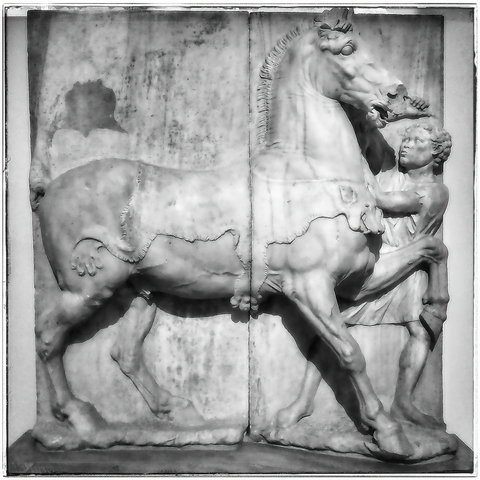
\includegraphics{smallthumb-lesson_I.jpeg}
\setfloatalignment{b}
\end{marginfigure}


\begin{abstract}
\noindent
Queste lezioni si articolano in \textsc{elementi grammaticali}, 
espressi sommariamente, seguiti da \textsc{vocabolari} per il lessico di base 
e da \textsc{frasi da tradurre} dal greco e in greco. 
\
L'approccio è quello del testo-laboratorio di morfosintassi: 
si presenta punto per punto - riprendendone la numerazione - 
l'esposizione di Gleason\cite{gleason1903}.\\
\bigskip
\noindent
Lezione XI: Ripasso dell'indicativo attivo, tema e temi temporali del verbo, perfetto secondo, vocabolario, esercizi.
\end{abstract}

%\printclassoptions

\newthought{133. Presente e Imperfetto.} Il \textit{tema (temporale) del presente} e dell'imperfetto sono uguali e si desumono dalla prima persona singolare del presente indicativo attivo. La sua vocale finale è \didobf{ο} prima di \didobf{μ} o \didobf{ν}, altrimenti è \didobf{ε}. 

\newthought{134. Futuro.} Il \textit{tema del futuro attivo e medio} si forma aggiungendo \didobf{-σο (-σε)} al tema \textit{(tema verbale, appunto)} del verbo\sidenote{I verbi in liquida hanno futuro e aoristo senza \didobf{σ}. Vedi (487.)}. 

\newthought{135. Aoristo Primo.} Il \textit{tema dell'aoristo primo attivo e medio} si forma aggiungendo \didobf{-σα} al tema del verbo.

\newthought{Osservazione}
\begin{itemize}
\item[\textsc{a.}] I temi verbali in linguale (\didobf{τ, δ, θ}) prima della \didobf{σ} la perdono, 
come in \didobf{πείθω}, \textit{persuadere,} fut. \didobf{πείσω}; \didobf{ἀθροίζω} (tema verbale \didobf{ἀθροιδ-}), \textit{raccogliere,} fut. \didobf{ἀθροισω}. 
\end{itemize}

\newthought{136. Aoristo Secondo.} Il \textit{tema dell'aoristo secondo} si forma aggiungendo \didobf{ο} o \didobf{ε (-ο/-ε)} al tema del verbo. All'indicativo, si coniuga come l'imperfetto, negli altri modi si coniuga come il presente. 

\newthought{137. Perfetto Primo.} Nei temi verbali in vocale, in molti temi in liquida e in alcuni temi in linguale il \textit{tema del perfetto (primo)} si forma aggiungendo \didobf{-κα} al tema verbale raddoppiato.

\hyphenation{θαυ-μά-ζω}

\newthought{Osservazione}
\begin{itemize}
\item[\textsc{1.}] Anche qui i temi verbali in linguale (\didobf{τ, δ, θ}, specialmente quelli con il presente in \didobf{-ζω}) prima della \didobf{κα} la perdono, come in \didobf{θαυμάζω} (tema verbale \didobf{θαυμαδ-}), \textit{ammirare,} perfetto \didobf{τεθαύμακα}.
\end{itemize}

\newthought{138. Perfetto Secondo.} Per formare il perfetto molti verbi aggiungono \didobf{α} al tema verbale raddoppiato. La maggior parte dei temi in \didobf{π, β, κ, γ}, se preceduta da vocale breve, la cambiano nella muta cognata aspra; i temi in \didobf{φ, χ} rimangono invariati. Per convenienza, questo perfetto viene chiamato \textit{perfetto secondo}, a distinguerlo da quello in \didobf{-κα}. La coniugazione è la medesima.
\newthought{Osservazione}
\begin{itemize}
\item[\textsc{a.}] I seguenti verbi, già incontrati in vocabolari precedenti, hanno perfetto secondo:
\begin{multicols}{2}
    \noindent \hangindent=1em \didobf{ἄγω}, pf. \didobf{ἦχα},  \\
	\noindent \hangindent=1em \didobf{γράφω}, pf. \didobf{γέγραφα},  \\
	\noindent \hangindent=1em \didobf{διώκω}, pf. \didobf{δεδίωχα},  \\
	
	\noindent \hangindent=1em \didobf{πέμπω}, pf. \didobf{πέπομφα},  \\
	\noindent \hangindent=1em \didobf{λείπω}, pf. \didobf{λέλοιπα},  \\
	\noindent \hangindent=1em \didobf{φεύγω}, pf. \didobf{πέφευγα}. 
\end{multicols}
\end{itemize}

\newthought{139. Piuccheperfetto Primo.} Il piuccheperfetto cambia la \didobf{-κα} del perfetto in \didobf{-κε}, che al singolare diviene \didobf{-κη, -κης, -κει(ν)}.
\sidenote{forma contratta dallo ionico \didobf{-κεα}, usata al posto del dialetto attico \didobf{-κειν}}

\newthought{140. Piuccheperfetto Secondo.} La vocale \didobf{α} del perfetto secondo diventa \didobf{ε} nel piuccheperfetto secondo; la coniugazione è la stessa del piuccheperfetto primo.

\newthought{Esercizio}
\begin{itemize}
\item[\textsc{a.}] Coniuga il piuccheperfetto dei verbi in (138, a). 
\end{itemize}

\newthought{141. Vocabolario}

\begin{multicols}{2}
    \noindent \hangindent=1em \didobf{κεφαλέ, ἡ} \textit{testa}.  \\
    \noindent \hangindent=1em \didobf{στρατηγός, ὁ} \textit{comandante, generale}.  \\
    \noindent \hangindent=1em \didobf{πολέμιος, α, ον} agg. \textit{ostile}.  \\
    \noindent \hangindent=1em \didobf{οἱ πολέμιοι} \textit{il nemico}.  \\
    \noindent \hangindent=1em \didobf{πολλοί, πολλαί, πολλά} agg. \textit{molti}.  \\

    \noindent \hangindent=1em \didobf{αφροίζω}, fut. \didobf{αφροίσω}, aor. \didobf{ἔφροισα}, pf. \didobf{ἔφροικα},	\textit{raccogliere.} \\ 
	\noindent \hangindent=1em \didobf{διδάσκω}, fut. \didobf{διδάξω}, aor. \didobf{ἐδίδαξα}, pf. \didobf{δεδίδακα},	\textit{insegnare.} \\ 
	\noindent \hangindent=1em \didobf{κλέπτω}, fut. \didobf{κλέψω}, aor. \didobf{ἔκλεψα}, pf. \didobf{κέκλοφα},	\textit{rubare.} \\ 
	\noindent \hangindent=1em \didobf{πείφω}, fut. \didobf{πείσω}, aor. \didobf{ἔπεισα}, pf. \didobf{πέπεικα}, \textit{persuadere.} \\ 
	\noindent \hangindent=1em \didobf{ρίπτω}, fut. \didobf{ρίφω}, aor. \didobf{ἔρριψα}, pf. \didobf{ἔρριφα}, \textit{lanciare.} \\ 
	
	\noindent \hangindent=1em \didobf{μετά}, prep. 
	con \gen \textit{con}; 
	con \acc \textit{dopo}. \\
	
	\noindent \hangindent=1em \didobf{ἀλλά}, cong. \textit{ma, ancora.} \\ 
	
\end{multicols}

\newthought{142. Traduci:}
\textsc{1.}~\dido{πείθουσιν, ἔπειθον, πείσουσιν.} \quad
\textsc{2.}~\dido{ἔπεισαν, πεπείκασιν, ἐπεπείκεσαν.} \quad
\textsc{3.}~\dido{ἠθροίσαμεν, διδάξει, ἦγε, κλέψετε.} \quad
\textsc{2.}~\dido{ἔρριφας, ἔλαβε, λέλοιπα, ἐδεδιδάχης.} \quad
\textsc{2.}~\dido{μένομεν, ἐβάλετε, ἦχεν, ἤχει.} \\

\hyphenation{ἐ-στρά-τευ-σεν}
\hyphenation{κλέ-ψου-σι}

\newthought{143.}
\textsc{1.}~\dido{ἐδίδαξαν τὰ τέκνα γράφειν λόγους σοφούς.} \quad
\textsc{2.}~\dido{ἐν δὲ τῇ στενῇ ὁδῷ ἠθροίκασι πολλοὺς δούλους.} \quad
\textsc{3.}~\dido{ἀλλὰ ταῖς λόγχαις ἔπαιον τὰς κεφαλὰς τῶν ἀγγέλων.} \quad
\textsc{4.}~\dido{ηὗρε δὲ τὸν ἀδελφὸν ἐν τῷ καπηλείῷ· οἶνον δὲ οὐκ ἔπινεν.} \quad
\textsc{5.}~\dido{ἐπὶ δὲ ταῖς τοῦ ποταμοῦ πηγαῖς ἔλιπε τὸ ἱμάτιον.} \quad
\textsc{6.}~\dido{ἐκεκελεύκει γὰρ τὰ παιδία ῤίπτειν τοὺς λίθους εἰς τὴν θάλατταν.} \quad
\textsc{7.}~\dido{ὁ δὲ στρατηγὸς εὐθὺς ἐστράτευσεν ἐπὶ τοὺς πολεμίους.} \quad
\textsc{8.}~\dido{άλλ´ἐπεὶ ἥρπασαν\sidenote{traduci come fosse piuccheperfetto.} τὰς κώμας ἔφυγον πολλὰ πλέθρα διὰ τοῦ πεδίου.} \quad
\textsc{9.}~\dido{μένουσιν ἐν τῷ ἱερῷ καὶ κλέψουσι τὰ τῶν Μουσῶν δῶρα.} \quad
\textsc{10.}~\dido{μακρὰ ἦν ἡ μάχη, ἀλλὰ καλὴ ἡ νίκη.} 

\newthought{144. Scrivi in Greco:}
\textsc{1.}~Ma ha mandatoil nemico alla cittadella.\quad
\textsc{2.}~E raccolsero molti carri riempiti con bei doni. \quad
\textsc{3.}~Perché avevano fatto una spedizione con il generale.


\begin{figure*}[!b]
  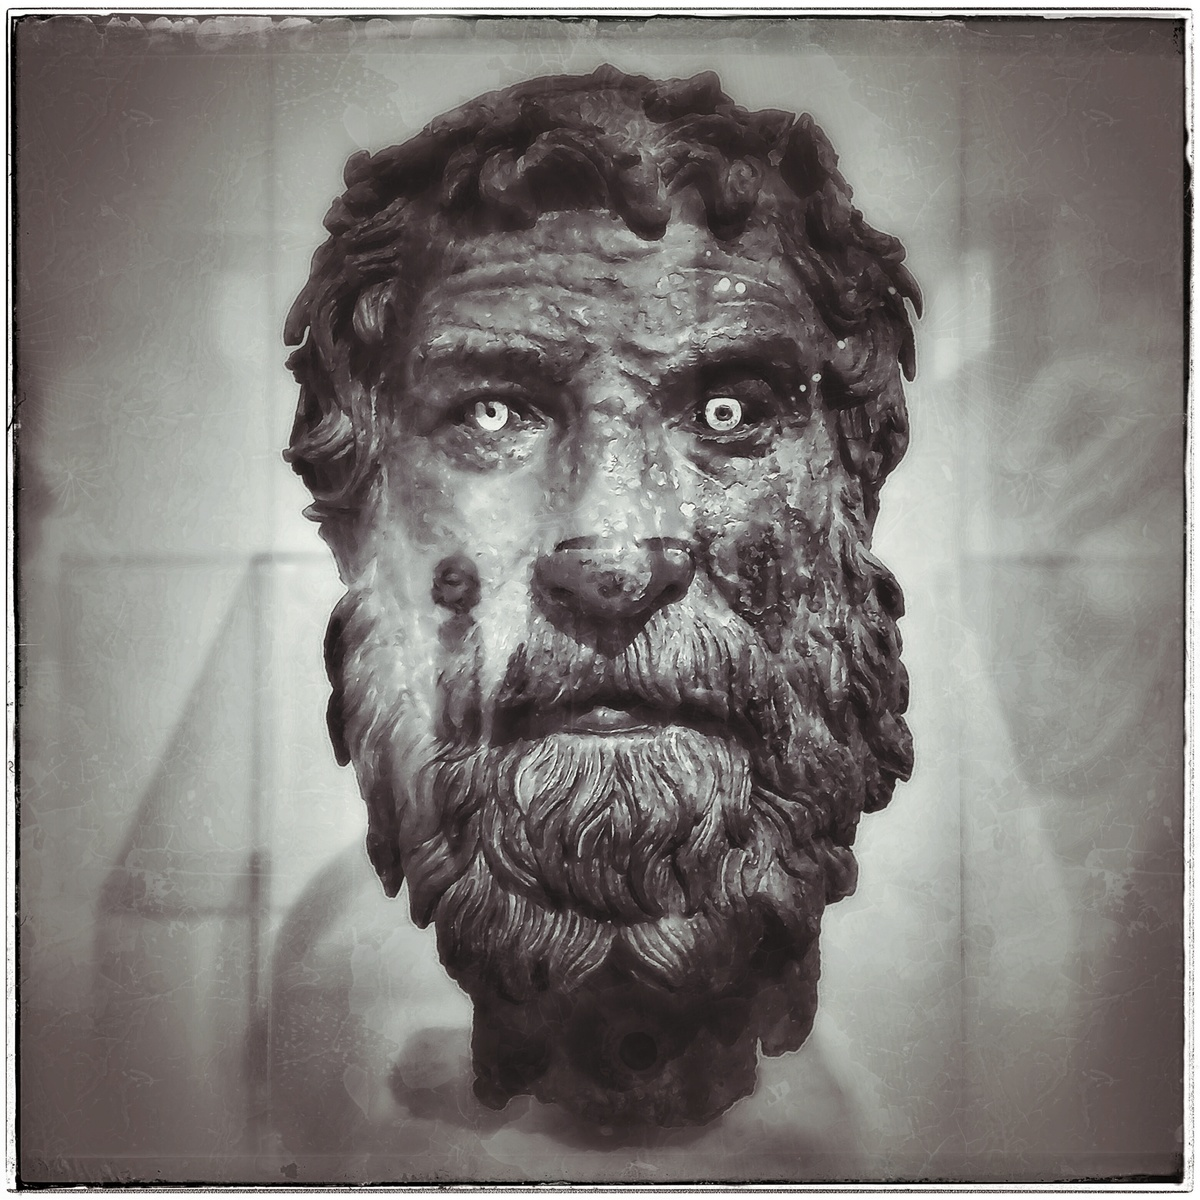
\includegraphics[width=0.7\linewidth]{thumb-lesson_XI.jpeg}´᾿
  %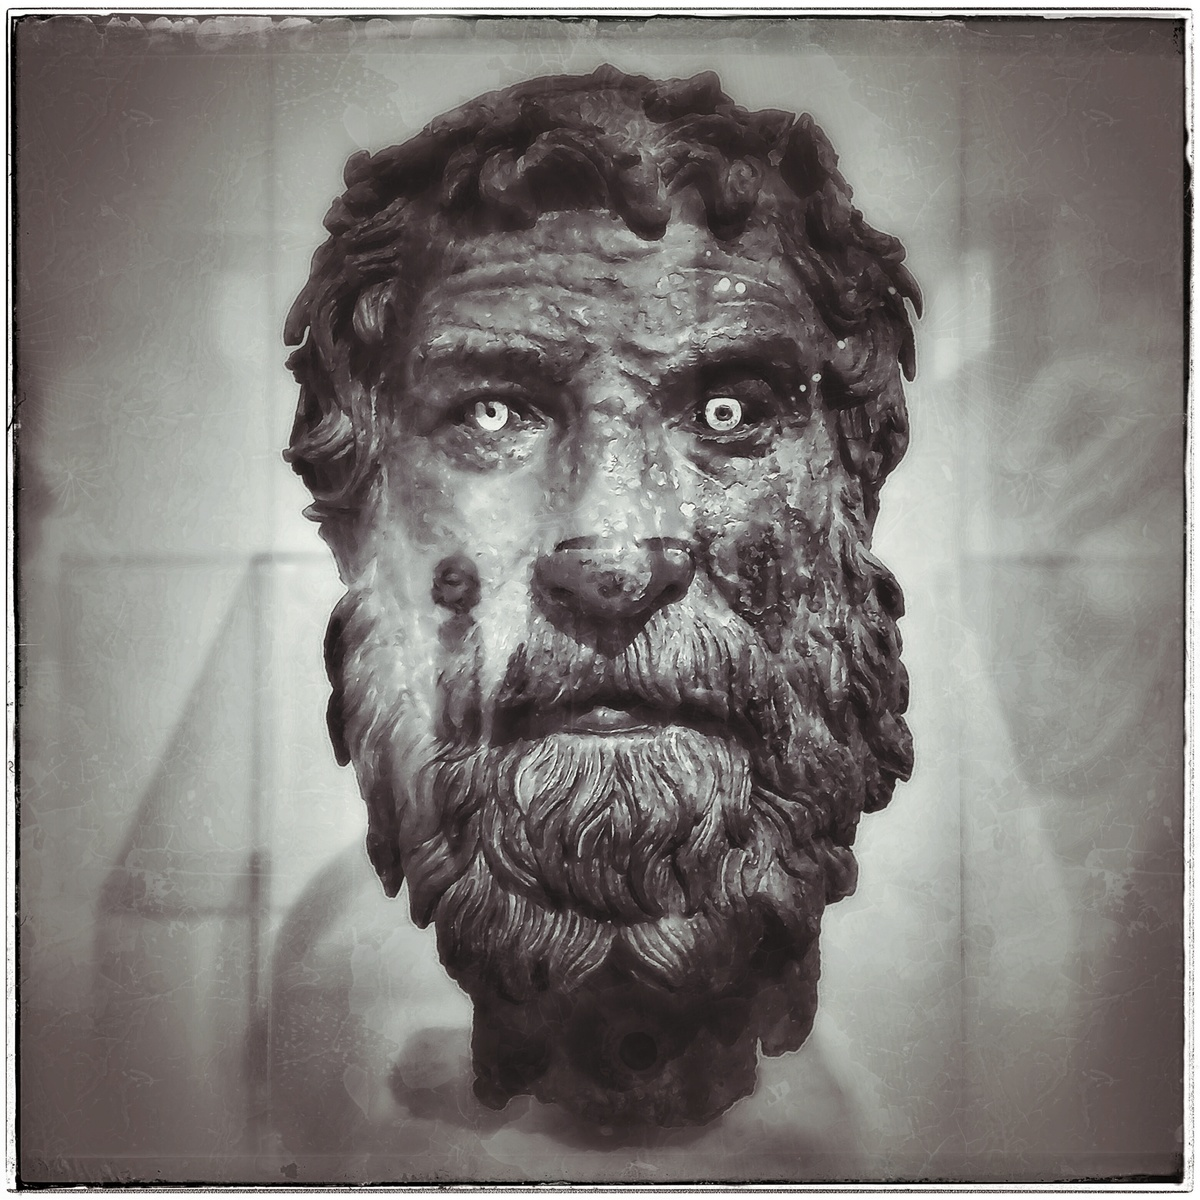
\includegraphics{thumb-lesson_XI.jpeg}
  \caption{Museo Nazionale di Archeologia di Atene}
  \label{fig:textfig}
  %\zsavepos{pos:textfig}
  %\setfloatalignment{b}
\end{figure*}

 

\nobibliography{greekBiblio}
\bibliographystyle{alpha}


\end{document}
